\documentclass[11pt]{article}
\usepackage[a4paper,margin=2.5cm]{geometry}
\usepackage{amsmath,amssymb,amsthm,graphicx,booktabs,xcolor}
\usepackage[colorlinks=true,linkcolor=blue!60!black,citecolor=blue!60!black,urlcolor=blue!60!black]{hyperref}
\hypersetup{pdftitle={Uncomputable Fractal Dimensions, Kolmogorov Complexity Cascades, and the Chaitin Barrier},pdfauthor={Ruqing Chen}}
\setlength{\emergencystretch}{2em}
\graphicspath{{../figures/}{figures/}{./}}

\newtheorem{theorem}{Theorem}
\newtheorem{proposition}{Proposition}[section]
\newtheorem{corollary}{Corollary}[section]
\newtheorem{lemma}{Lemma}[section]
\theoremstyle{definition}\newtheorem{definition}{Definition}[section]
\theoremstyle{remark}\newtheorem*{remark}{Remark}

\newcommand{\dd}{\mathrm{d}}
\newcommand{\NN}{\mathbb{N}}
\newcommand{\Kc}{K}

\title{Uncomputable Fractal Dimensions,\\ Kolmogorov Complexity Cascades,\\ and the Chaitin Barrier in Physical Systems}
\author{Ruqing Chen\\[2pt]
\small GUT Geoservice Inc., Montreal, Quebec, Canada\\
\small \href{mailto:ruqing@hotmail.com}{\texttt{ruqing@hotmail.com}}}
\date{\small DOI: \href{https://doi.org/10.5281/zenodo.23194419}{10.5281/zenodo.23194419}}

\begin{document}
\maketitle

\begin{abstract}
We study three questions at the interface of fractal geometry and algorithmic information theory.

First, we construct a computable compact set $\mathcal K\subset[0,1]$ whose box-counting and Hausdorff
dimensions both equal $\frac14+\frac12\Omega$, where $\Omega$ is Chaitin's halting probability. The dimension is
therefore left-computably-enumerable but not computable. The construction is a homogeneous Cantor set
with stage-dependent ratios driven by computable lower approximations of $\Omega$, and the dimension follows from
a Ces\`aro argument and the mass distribution principle. We also check the limits of the construction: no
self-similar set with finitely many computable ratios can have an uncomputable dimension, and the known
non-computability of certain Julia sets concerns the sets rather than their dimensions.

Second, we classify the growth of the Kolmogorov complexity of $\varepsilon$-discretisations with
$L=\ln(1/\varepsilon)$ into three tiers. It is $\Theta(\log L)$ for every computable set, including smooth
manifolds, self-similar fractals and the set above; $\Theta(L)$ when one incompressible symbol is injected per
scale; and $e^{\Theta(L)}$ for independent randomness in every cell. Every question about a finite
discretisation is decidable, and undecidability enters only through limits, as in the undecidability of the
spectral gap.

Third, we test quantitatively the idea that physical cutoffs act as a ``firewall'' protecting physics from
G\"odel incompleteness, and find that the numbers refute it. Independence from ZFC already occurs for a
Turing machine whose description is of order $10^5$ bits, while a macroscopic crystal at atomic resolution
carries up to $10^{24}$ bits of configurational information, and even a one-dimensional random fractal
crosses the barrier at $L^*\approx34.5$, far above the Planck scale ($L_P\approx80$ for a 1\,m system).

Numerical illustrations use binary lambda calculus, whose closed-term counts reproduce OEIS A114852, and
LZMA compression of four classes of Cantor-type sets.
\end{abstract}

\tableofcontents

%=====================================================================
\section{Introduction}
\label{sec:intro}

Self-similarity is usually associated with simplicity: a finite iterated function system (IFS) describes a
fractal with infinitely many details by a few numbers, and its dimension follows from a single equation. On the
other hand, algorithmic information theory~\cite{LiVitanyi,DowneyHirschfeldt} distinguishes real numbers and
infinite objects that can be computed to arbitrary precision from those that cannot. The canonical
uncomputable real is Chaitin's halting probability~\cite{Chaitin75}
\begin{equation}
\Omega=\sum_{p\in\mathrm{dom}(U)}2^{-|p|},
\end{equation}
where $U$ is a universal prefix-free machine. $\Omega$ is left-computably-enumerable (left-c.e.): it is the limit
of a computable non-decreasing sequence of rationals $\Omega_s$. However, it has no computable modulus of
convergence, and its binary expansion is Martin-L\"of random~\cite{MartinLof,Chaitin75}.

This paper asks three questions.
\begin{enumerate}
\item Can a set that a computer draws to any desired precision have an uncomputable fractal dimension?
\item How does the Kolmogorov complexity of an $\varepsilon$-discretised geometric object grow as
$\varepsilon\to0$, and where, if anywhere, does undecidability enter?
\item Are physical cutoffs, such as the Planck length or a lattice spacing, needed to protect physical laws from
G\"odel incompleteness and the halting problem?
\end{enumerate}
Our answers are: yes, with an explicit construction and proof (Section~\ref{sec:construction}); a three-tier
classification, with undecidability confined to limits (Section~\ref{sec:tiers}); and no, by a quantitative
argument (Section~\ref{sec:firewall}). Section~\ref{sec:numerics} presents numerical illustrations, and
Section~\ref{sec:discussion} discusses scope and limitations.

\paragraph{Related work.} Non-computable quadratic Julia sets were constructed by Braverman and
Yampolsky~\cite{BY}. Undecidability of a physical property, the spectral gap of a translationally invariant
lattice Hamiltonian, was proved by Cubitt, P\'erez-Garc\'ia and Wolf~\cite{CPW}, and Moore showed that
low-dimensional dynamical systems can be computationally universal, which makes long-time questions
undecidable~\cite{Moore}. Chaitin's information-theoretic incompleteness theorem bounds the complexity that a
formal system can certify~\cite{Chaitin74}, and Yedidia and Aaronson gave an explicit 7910-state Turing
machine whose behaviour is independent of ZFC~\cite{YA}. For concrete prefix-free machines see Tromp's binary
lambda calculus~\cite{Tromp} and Stay~\cite{Stay}.

%=====================================================================
\section{A computable set with uncomputable fractal dimension}
\label{sec:construction}

\subsection{Statement}
A compact set $\mathcal K\subset\mathbb R$ is \emph{computable} if there is an algorithm that, given $k$, outputs a
finite union of rational intervals whose Hausdorff distance to $\mathcal K$ is at most $2^{-k}$~\cite{Weihrauch}.

\begin{theorem}
\label{thm:main}
Let $(\Omega_s)_{s\ge1}$ be a computable non-decreasing sequence of rationals in $[0,1)$ converging to $\Omega$.
Put $d_k=\frac14+\frac12\Omega_k$ and $r_k=2^{-1/d_k}$. Let $\mathcal K=\bigcap_kE_k$, where $E_0=[0,1]$ and $E_k$ is obtained
from $E_{k-1}$ by replacing every interval $I$ by its two end pieces of length $r_k|I|$. Then $\mathcal K$ is a computable
compact set and
\begin{equation}
\dim_B\mathcal K=\dim_H\mathcal K=D\equiv\tfrac14+\tfrac12\Omega .
\end{equation}
In particular $\dim_H\mathcal K$ is left-c.e.\ but not computable.
\end{theorem}

\subsection{Proof}
Since $\Omega_k\in[0,1)$, we have $d_k\in[\frac14,\frac34)$ and
\begin{equation}
r_k\in\big[2^{-4},\,2^{-4/3}\big),\qquad 1-2r_k>1-2^{-1/3}>0.206 .
\label{eq:bounds}
\end{equation}
Write $\delta_k=\prod_{j\le k}r_j$, the common length of the $2^k$ intervals of $E_k$.

\emph{Computability.} Each $E_k$ is a finite union of intervals whose endpoints are computable reals, uniformly in
$k$. Every interval of $E_k$ contains points of $\mathcal K$, and $\mathcal K\subset E_k$, so the Hausdorff distance between $E_k$ and
$\mathcal K$ is at most $\delta_k\le2^{-4k/3}$. Rational approximations of the endpoints to within $2^{-k}$ therefore give
the required approximations, and $\mathcal K$ is computable.

\emph{Box dimension.} Two intervals of $E_k$ with the same parent are separated by a gap of length
$(1-2r_k)\delta_{k-1}\ge0.206\,\delta_{k-1}$, and gaps created at earlier stages are larger. For
$\delta_k\le\delta<\delta_{k-1}$, each interval of $E_k$ meets at most two $\delta$-mesh cells, so
$N_\delta(\mathcal K)\le2^{k+1}$. Conversely, the $2^{k-1}$ intervals of $E_{k-1}$ are separated by gaps of at least
$0.206\,\delta_{k-2}\ge0.206\,\delta$, so each $\delta$-cell meets at most a bounded number $C$ of them and
$N_\delta(\mathcal K)\ge2^{k-1}/C$. Since $r_k\ge2^{-4}$, $\ln(1/\delta)=\ln(1/\delta_k)+O(1)$. Hence
\begin{equation}
\dim_B\mathcal K=\lim_{k\to\infty}\frac{k\ln2}{\ln(1/\delta_k)}=\lim_{k\to\infty}\frac{k\ln2}{\sum_{j\le k}\ln2/d_j}
=\lim_{k\to\infty}\Big(\frac1k\sum_{j\le k}\frac1{d_j}\Big)^{-1}=D,
\end{equation}
because $1/d_j\to1/D$ and Ces\`aro means of a convergent sequence converge to the same limit.

\emph{Hausdorff dimension.} Let $\mu$ be the natural measure, giving mass $2^{-k}$ to every interval of $E_k$. For a
ball $B$ of radius $\delta$ with $\delta_{k+1}\le\delta<\delta_k$, the gaps between intervals of $E_k$ are at least
$0.206\,\delta_{k-1}\ge0.206\,\delta_k$, so $B$ meets at most $M=\lceil2/0.206\rceil+2=12$ of them. Hence
$\mu(B)\le12\cdot2^{-k}$. Given $\eta>0$, for large $k$ we have $2^{-k}\le\delta_{k+1}^{\,D-\eta}\le\delta^{D-\eta}$ by the box-dimension
computation, so $\mu(B)\le12\,\delta^{D-\eta}$. The mass distribution principle~\cite{Falconer} gives
$\dim_H\mathcal K\ge D-\eta$ for every $\eta>0$. Together with $\dim_H\le\dim_B=D$, this proves $\dim_H\mathcal K=D$.

\emph{Uncomputability.} If $D$ were computable, so would be $\Omega=2D-\frac12$, contradicting the uncomputability of
$\Omega$~\cite{Chaitin75}. $D$ is left-c.e.\ because $\Omega$ is. \hfill$\square$

\subsection{Scope of the construction}
\begin{proposition}[Self-similar sets have computable dimension]
\label{prop:selfsim}
Let $\mathcal K$ be the attractor of a finite IFS of similarities with computable ratios $r_1,\dots,r_N$ satisfying the
open set condition. Then $\dim_H\mathcal K=\dim_B\mathcal K$ is computable.
\end{proposition}
\begin{proof}
The dimension is the unique root $s$ of $\sum_ir_i^s=1$~\cite{Hutchinson,Falconer}. The function $s\mapsto\sum_ir_i^s$ is
computable and strictly decreasing, so the root can be computed to any precision by bisection.
\end{proof}
Uncomputability of the dimension therefore requires infinitely many independent data, as in
Theorem~\ref{thm:main}, where the ratios change at every stage.

\begin{remark}[Julia sets]
Braverman and Yampolsky proved that there exist quadratic Julia sets that are not computable~\cite{BY}. That
result concerns computability of the \emph{set}. It is logically independent of Theorem~\ref{thm:main}, in which
the set is computable but its dimension is not.
\end{remark}

\begin{remark}[Information content]
The set of Theorem~\ref{thm:main} has small Kolmogorov complexity at every finite resolution
(Proposition~\ref{prop:tier1}). The uncomputable information resides only in the limit $k\to\infty$. Since the
convergence $\Omega_s\to\Omega$ has no computable modulus, no algorithm can certify the dimension to a prescribed
precision from finite-resolution data.
\end{remark}

%=====================================================================
\section{Three-tier hierarchy of Kolmogorov complexity under scaling}
\label{sec:tiers}

Let $S_\varepsilon$ be the binary image of a set on the $\varepsilon$-grid of $[0,1]^n$, with $\varepsilon=2^{-k}$, and let
$L=\ln(1/\varepsilon)=k\ln2$. Let $\Kc(\cdot)$ denote prefix Kolmogorov complexity~\cite{LiVitanyi}.

\begin{proposition}[Tier 1: computable sets]
\label{prop:tier1}
For every computable compact set $\mathcal K$ (and a fixed rule for discretising it),
\begin{equation}
\Kc(S_\varepsilon)\le\Kc(k)+O(1)\le\log_2L+2\log_2\log_2L+O(1),
\end{equation}
and $\Kc(S_\varepsilon)\ge\Kc(k)-O(1)$, so $\Kc(S_\varepsilon)=\Theta(\log L)$ for all but a sparse set of $k$. This
applies to smooth manifolds, to self-similar fractals and to the set of Theorem~\ref{thm:main}.
\end{proposition}
\begin{proof}
A fixed program that computes $\mathcal K$, given $k$, outputs $S_{2^{-k}}$, which proves the upper bound. Conversely, $k$ can be read
off from the size of $S_\varepsilon$, so $\Kc(k)\le\Kc(S_\varepsilon)+O(1)$, and $\Kc(k)\ge\log_2k$ for most $k$.
\end{proof}

\begin{proposition}[Tier 2: one incompressible symbol per scale]
\label{prop:tier2}
Let the ratio at stage $j$ of a homogeneous Cantor construction be chosen from two fixed values according to the
$j$-th bit $x_j$ of an infinite binary sequence $x$. If $x$ is Martin-L\"of random (for instance
$x=\Omega$), then $\Kc(S_\varepsilon)=k\,\Theta(1)+O(\log k)$, i.e.\ $\Theta(L)$.
\end{proposition}
\begin{proof}
The first $k$ bits of $x$ can be recovered from the stage-$k$ image, because the stage-$j$ ratio is read off from
the gap structure. Hence $\Kc(x\!\upharpoonright\!k)\le\Kc(S)+O(\log k)$. Martin-L\"of randomness gives
$\Kc(x\!\upharpoonright\!k)\ge k-O(1)$~\cite{Chaitin75,DowneyHirschfeldt}. The upper bound $\Kc(S)\le k+O(\log k)$ follows
from describing $x\!\upharpoonright\!k$ literally. The resolution at stage $k$ satisfies $L=\Theta(k)$.
\end{proof}
Such a set is not computable, because it computes $x$.

\begin{proposition}[Tier 3: independent randomness per cell]
\label{prop:tier3}
If every interval chooses its own ratio by an independent fair bit, then with probability at least $1-2^{-c}$
one has $\Kc(S_\varepsilon)\ge N_\varepsilon-c$, where $N_\varepsilon\sim\varepsilon^{-D}=e^{DL}$ is the number of decision bits
up to resolution $\varepsilon$.
\end{proposition}
\begin{proof}
The map from decision bits to images is injective, and at most $2^{N-c}$ strings of length $N$ have complexity
below $N-c$.
\end{proof}

\paragraph{Decidability at finite resolution.} Every question about a fixed $S_\varepsilon$ is a question about a
finite object and is therefore decidable. Complexity classes such as NP-hardness describe how cost scales with
the size of the input. They do not describe a threshold resolution $\varepsilon^*$ below which a problem suddenly
becomes hard. Undecidability enters only through questions that quantify over all scales or all sizes. In the
spectral-gap construction of~\cite{CPW}, whether the system is gapped depends on whether a universal Turing
machine halts, and the finite-size behaviour can mimic the opposite phase up to system sizes that admit no
computable bound. The precise form of the ``critical scale'' intuition is therefore: \emph{for each instance a
crossover scale exists, but it is not a computable function of the instance.}

%=====================================================================
\section{Quantitative refutation of a ``Planck firewall'' against G\"odel}
\label{sec:firewall}

One may conjecture that a discrete physical cutoff, Planck or atomic, protects physical laws from G\"odel
incompleteness by halting the growth of algorithmic complexity before it reaches Chaitin's barrier. We argue
that this conjecture fails on four counts.

\paragraph{1. Logic.} Incompleteness and the halting problem limit what a formal system can prove and what an
algorithm can decide. They do not render physical laws inconsistent. A physical state whose properties are
unprovable in a given theory is not a paradox.

\paragraph{2. Cutoffs do not remove undecidability.} The spectral-gap problem is undecidable for Hamiltonians
defined \emph{on a lattice}, i.e.\ with a cutoff already in place~\cite{CPW}. The undecidability comes from the
thermodynamic limit. Moore's universal dynamical systems with three degrees of freedom are undecidable through
the infinite-time limit~\cite{Moore}. Removing short distances leaves both limits intact.

\paragraph{3. The barrier is crossed long before any cutoff.} By Chaitin's incompleteness theorem, a formal system
$F$ cannot prove $\Kc(x)>c_F$ for any specific $x$, where $c_F$ is of the order of the complexity of
$F$~\cite{Chaitin74}. Yedidia and Aaronson exhibited a 7910-state, two-symbol Turing machine whose halting is
independent of ZFC~\cite{YA}. Encoding each of its $2\times7910$ transitions with about 15 bits gives an
illustrative scale
\begin{equation}
c_F\approx2.4\times10^5\ \text{bits}.
\end{equation}
By comparison:
\begin{itemize}
\item a $1\,\mathrm{cm}^3$ crystal at atomic resolution ($1$\,\AA) has $10^{24}$ sites, so its configurational
information can reach $10^{24}$ bits;
\item even the one-dimensional tier-3 random Cantor set of Section~\ref{sec:numerics}, with $D\approx0.36$, reaches
$\Kc\sim e^{DL}=c_F$ at $L^*=\ln c_F/D\approx34.5$, i.e.\ at $\varepsilon^*\approx10^{-15}$ of the system size;
\item the Planck cutoff for a $1$\,m system corresponds to $L_P=\ln(1\,\mathrm m/1.6\times10^{-35}\,\mathrm m)\approx80$.
\end{itemize}
The premise that cutoffs come before the barrier is therefore false by many orders of magnitude.

\paragraph{4. The barrier has no dynamical content.} Exceeding $c_F$ changes nothing in the evolution of a
system. It only limits which statements about its description $F$ can prove.

\paragraph{A defensible weaker statement.} If both an ultraviolet and an infrared cutoff hold, so that the
relevant Hilbert space is finite-dimensional, then every question about a finite region over a finite time is
decidable in principle. Undecidability in physics then arises only from idealised infinite limits. This
follows from finiteness of the information content and has no relation to G\"odel's theorem.

%=====================================================================
\section{Numerical illustrations}
\label{sec:numerics}

\subsection{A toy halting probability in binary lambda calculus}
In binary lambda calculus (BLC)~\cite{Tromp}, a term in de Bruijn notation is encoded as $00M$ for an
abstraction $\lambda M$, $01MN$ for an application $MN$, and $1^{i+1}0$ for the variable with index $i$. The
encoding of closed terms is self-delimiting, so the set of closed-term codes is prefix-free. We define
\begin{equation}
\Omega_{\rm BLC}=\sum_{\text{closed }M\text{ with a }\beta\text{-normal form}}2^{-|M|},
\end{equation}
which is a left-c.e.\ real. We do not claim that it is Martin-L\"of random, which would require an optimal
universal prefix-free machine.

Our enumeration produces the numbers of closed terms of length $n=4,5,\dots,24$:
$1,0,1,1,2,1,6,5,13,14,37,44,101,134,298,431,883,1361,2736,4405,8574$. This agrees term by term with OEIS
A114852~\cite{OEIS}, which independently checks the enumerator. Normal-order reduction with a budget of 400
$\beta$-steps and $3000$ nodes certifies normalisation for all but $34$ of the $19\,048$ terms of length at most 24,
namely $1$, $1$, $7$ and $25$ undecided terms at lengths $18$, $20$, $22$ and $24$. This gives the rigorous lower bound
\begin{equation}
\Omega_{\rm BLC}\ge0.1201817393\ldots
\end{equation}

\paragraph{Why no bits are certified.} An upper bound requires bounding (a) the Kraft mass of all closed terms
longer than the enumeration, and (b) the mass of enumerated terms that never normalise. Our computation
provides neither. Without an analytic bound on the total closed-term measure, the remainder (a) can only be bounded
by $1-\sum_{|M|\le24}2^{-|M|}$. Without proofs of non-termination, the undecided terms in (b) must be counted as
possibly halting. The resulting upper bound is then trivially $1$, and no leading bit of $\Omega_{\rm BLC}$ is
certified. This is the general situation. More computation improves lower bounds, but each further certified bit
of a halting probability requires \emph{proofs} that specific programs do not halt, and Chaitin's theorem
limits how many such proofs any fixed formal system can supply~\cite{Chaitin74}.

\subsection{Complexity and dimension of four Cantor-type sets}
We rasterised four constructions on $2^{22}$ pixels of $[0,1]$. Each construction replaces every interval by its
two end pieces:
\begin{enumerate}
\item self-similar, $r=1/4$ (tier 1);
\item $r_k=2^{-1/d_k}$ with $d_k=\frac14+\frac12\Omega_k$, using the BLC lower bounds as $\Omega_k$ (tier 1, by
Proposition~\ref{prop:tier1});
\item one random bit per stage selecting $r_k\in\{0.25,0.10\}$, a stand-in for the bits of $\Omega$ (tier 2);
\item one random bit per interval (tier 3).
\end{enumerate}
For each stage we record the LZMA-compressed size~\cite{ZivLempel} minus that of an empty bitmap ($1664$ bits), which is
an upper bound on $\Kc$ up to an additive constant, together with the box-counting dimension.

The results are shown in Fig.~\ref{fig:chaitin}. The self-similar set saturates at about $10^3$ bits for $L\gtrsim8$. The
tier-3 set grows fastest, reaching about $3\times10^3$ bits at stage 7 with $128$ intervals, and the tier-2 set lies in
between. LZMA can only approximate the true complexities from above: it cannot discover the $O(\log L)$ programs
of tier-1 sets. The box-counting dimension of construction 2 approaches the Ces\`aro value of the stage ratios
($0.29$ at stage 6, against $0.31$ from box counting). The limiting dimension $\frac14+\frac12\Omega_{\rm BLC}$ is known
only to lie in $[0.310,0.75]$.

\begin{figure}[t]
\centering
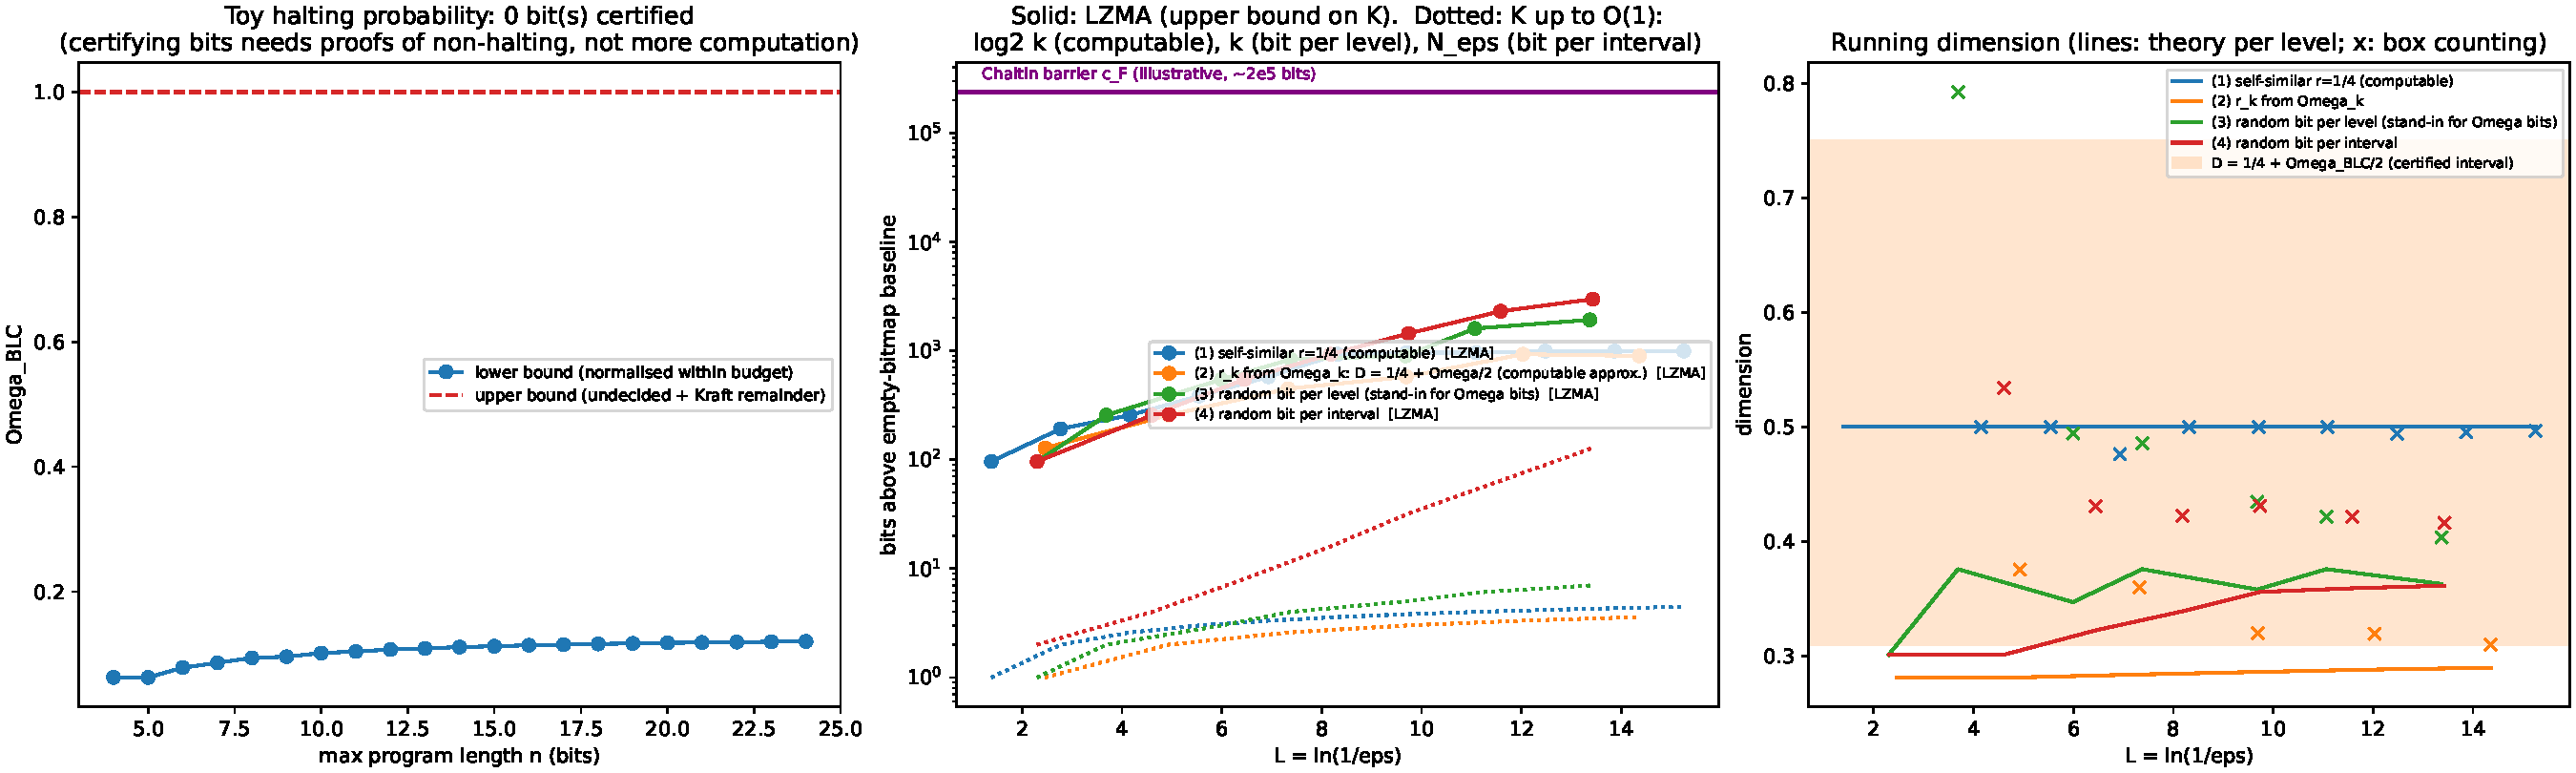
\includegraphics[width=\textwidth]{chaitin_fractal}
\caption{Left: lower bound on the toy halting probability $\Omega_{\rm BLC}$ against the maximal program length; the
upper bound is trivial (see text). Middle: LZMA-compressed size above the empty-bitmap baseline (solid) and the
complexity predicted by Propositions~\ref{prop:tier1}--\ref{prop:tier3} up to $O(1)$ (dotted) for the four
constructions; the horizontal line marks the illustrative Chaitin scale $c_F$. Right: running dimension per
stage (lines) and box-counting estimates (crosses); the band is the interval for
$\frac14+\frac12\Omega_{\rm BLC}$ implied by the bounds on $\Omega_{\rm BLC}$.}
\label{fig:chaitin}
\end{figure}

%=====================================================================
\section{Discussion and physical scope}
\label{sec:discussion}
\begin{enumerate}
\item Theorem~\ref{thm:main} uses a universal prefix-free machine only through the left-c.e.\ real $\Omega$. Any
left-c.e.\ real in $[0,1)$ can be substituted, so the construction realises every left-c.e.\ dimension in
$[\frac14,\frac34)$. Extending it to other classes of reals, or to dimensions of sets defined by natural dynamics,
is left open.
\item Proposition~\ref{prop:tier1} shows that uncomputability of a geometric invariant is compatible with
minimal complexity at every finite resolution. The two notions should not be conflated.
\item The constant $c_F\approx2.4\times10^5$ bits is illustrative. Smaller ZFC-independent machines have since been
reported, which only strengthens the argument of Section~\ref{sec:firewall}.
\item The numerical part is illustrative: LZMA gives upper bounds only, and the BLC computation gives a lower bound
only, for a halting probability that we do not claim to be random.
\item Algorithmic complexity under scaling provides an information-theoretic foundation for the author's
broader programme of scale-dependent analysis (``pan-scale analytics'), complementing the geometric scaling in
holographic entanglement~\cite{Chen2026_holo} and the multifractal cascades in quantum many-body
systems~\cite{Chen2026_multi}.
\end{enumerate}

\section*{Data and code availability}
All numbers and Fig.~\ref{fig:chaitin} are produced by the Python script \texttt{chaitin\_fractal.py}, available
at \url{https://github.com/Ruqing1963/chaitin-fractal-complexity} and archived on Zenodo under DOI
\href{https://doi.org/10.5281/zenodo.23194419}{10.5281/zenodo.23194419}.

\appendix
\section{Technical details}
\label{app:tech}

\paragraph{BLC enumeration and reduction.} Terms of length exactly $s$ with free indices below $k$ are generated
recursively. A variable with index $i<k$ has length $i+2$, an abstraction has length $2+$ that of its body (with
$k\to k+1$), and an application has length $2+$ the sum of the lengths of its parts. Closed terms are those with
$k=0$. Reduction uses de Bruijn shifting and substitution with the leftmost-outermost (normal-order) strategy,
which finds a normal form whenever one exists. A term is recorded as normalising if no redex remains within 400
steps; it is recorded as undecided if the step budget is exhausted or the term exceeds 3000 nodes.

\paragraph{Lower and upper bounds.} The lower bound sums $2^{-|M|}$ over certified normalising terms. The upper
bound adds the mass of undecided terms and the Kraft remainder $1-\sum_{|M|\le n}2^{-|M|}$. Because every enumerated
term is either certified or undecided, this upper bound equals $1$ identically. A non-trivial upper bound requires
the two ingredients described in Section~\ref{sec:numerics}.

\paragraph{Rasterisation and compression.} Intervals are painted onto a uint8 array of $2^{22}$ cells using a
difference array, then bit-packed and compressed with LZMA (preset 9, extreme). The empty-bitmap baseline of $1664$
bits is subtracted. Construction stops once the smallest interval is shorter than one pixel.

\paragraph{Box counting.} Occupied boxes are counted at dyadic sizes $2^{-j}$, for $j=3,\dots,22$, restricted to box
sizes not smaller than the current stage length. The dimension is the least-squares slope of $\ln N$ against
$j\ln2$.

\begin{thebibliography}{99}
\bibitem{LiVitanyi} M.~Li, P.~Vit\'anyi, \emph{An Introduction to Kolmogorov Complexity and Its Applications}, 4th ed., Springer (2019).
\bibitem{DowneyHirschfeldt} R.~G.~Downey, D.~R.~Hirschfeldt, \emph{Algorithmic Randomness and Complexity}, Springer (2010).
\bibitem{Chaitin75} G.~J.~Chaitin, ``A theory of program size formally identical to information theory'', J.\ ACM 22 (1975) 329--340, doi:10.1145/321892.321894.
\bibitem{MartinLof} P.~Martin-L\"of, ``The definition of random sequences'', Inform.\ Control 9 (1966) 602--619.
\bibitem{BY} M.~Braverman, M.~Yampolsky, ``Non-computable Julia sets'', J.\ Amer.\ Math.\ Soc.\ 19 (2006) 551--578, doi:10.1090/S0894-0347-05-00516-3.
\bibitem{CPW} T.~S.~Cubitt, D.~P\'erez-Garc\'ia, M.~M.~Wolf, ``Undecidability of the spectral gap'', Nature 528 (2015) 207--211, doi:10.1038/nature16059, arXiv:1502.04135.
\bibitem{Moore} C.~Moore, ``Unpredictability and undecidability in dynamical systems'', Phys.\ Rev.\ Lett.\ 64 (1990) 2354.
\bibitem{Chaitin74} G.~J.~Chaitin, ``Information-theoretic limitations of formal systems'', J.\ ACM 21 (1974) 403--424.
\bibitem{YA} A.~Yedidia, S.~Aaronson, ``A relatively small Turing machine whose behavior is independent of set theory'', Complex Systems 25 (2016) 297, doi:10.25088/ComplexSystems.25.4.297, arXiv:1605.04343.
\bibitem{Tromp} J.~Tromp, ``Binary lambda calculus and combinatory logic'', in \emph{Randomness and Complexity: From Leibniz to Chaitin}, World Scientific (2007) 237--260, doi:10.1142/9789812770837\_0014.
\bibitem{Stay} M.~Stay, ``Very simple Chaitin machines for concrete AIT'', Fundam.\ Inform.\ 68 (2005) 231--247, arXiv:cs/0508056.
\bibitem{Weihrauch} K.~Weihrauch, \emph{Computable Analysis: An Introduction}, Springer (2000).
\bibitem{Falconer} K.~Falconer, \emph{Fractal Geometry: Mathematical Foundations and Applications}, 2nd ed., Wiley, Chichester (2003), doi:10.1002/0470013850.
\bibitem{Hutchinson} J.~E.~Hutchinson, ``Fractals and self similarity'', Indiana Univ.\ Math.\ J.\ 30 (1981) 713, doi:10.1512/iumj.1981.30.30055.
\bibitem{OEIS} OEIS Foundation, The On-Line Encyclopedia of Integer Sequences, sequence A114852, ``The number of closed lambda calculus terms of size $n$'', \url{https://oeis.org/A114852}.
\bibitem{ZivLempel} J.~Ziv, A.~Lempel, ``A universal algorithm for sequential data compression'', IEEE Trans.\ Inf.\ Theory 23 (1977) 337--343.
\bibitem{Chen2026_holo} R.~Chen, ``Holographic entanglement of fractal regions: Complex dimensions, non-local counterterms and cosmic-brane multifractality'' (2026), doi:10.5281/zenodo.23189575.
\bibitem{Chen2026_multi} R.~Chen, ``Multifractal large deviations in quantum entanglement: Ideal Fermi-gas mapping, Markov tensor cascades, and quartic Casimir symmetry'' (2026), doi:10.5281/zenodo.23193512.
\end{thebibliography}
\end{document}
